\chapter{System wizyjny zrealizowany na platformie Zynq z systemem operacyjnym PetaLinux}
\label{cha:project}


W ramach pracy zbadano możliwość realizacji systemów wizyjnych wykorzystujących możliwości obliczeniowe logiki programowalnej oraz procesora ARM i integrujących obie architektury w jednym procesie algorytmicznym. 
Zaproponowano moduł segmentacji obiektów pierwszoplanowych oparty o tzw. generację i modelowanie tła. 
Dane wejściowe pochodziły z kamery wideo połączonej z układem przy użyciu interfejsu HDMI. 
Sygnał wizyjny poddawany był przetwarzaniu i analizie przez elementy logiki programowalnej, a wyniki przesyłane były przy użyciu mechanizmu AXI VDMA do układu CPU. 
Proces rozpoznawania miał na celu indeksację obiektów pierwszoplanowych, z wykorzystaniem biblioteki OpenCV i procedury \texttt{cv::connectedComponents}. 
Wykorzystano ponadto mechanizm AXI DMA do konfiguracji parametrów algorytmu logiki programowalnej oraz wykorzystano narzędzia systemu operacyjnego PetaLinux do obsługi tego procesu. 
Zaproponowano również mechanizm synchronizacji dwóch kolejnych ramek sygnału przy użyciu modułu AXI VDMA.
Algorytm i jego podział na część sprzętową i programową przedstawiono na schemacie \ref{fig:full-algo}.

\begin{figure}[h]
	\centering
	\def\svgwidth{\textwidth}
	\input{img/full-algo.pdf_tex}
	\caption{Schemat algorytmu i podział na część sprzętową i programową.}
	\label{fig:full-algo}
\end{figure}

W przypadku algorytmów przetwarzania sekwencji obrazów, na etapie analizy jednej klatki wykorzystać można informacje uzyskane w trakcie obliczeń dla poprzednich ramek. 
Rozszerzenie kontekstu o parametry historyczne pozwala na projektowanie bardziej zaawansowanych systemów, zwykle wymaga jednak wykorzystania modułów zewnętrznej pamięci w celu przechowywania danych historycznych.

Wśród algorytmów wymagających kontekstu związanego z więcej niż jedną ramką obrazu wyróżnić można między innymi:
\begin{itemize}
	\item segmentację obiektów pierwszoplanowych -- umożliwia podział obrazu na elementy tła oraz znajdujące się na pierwszym planie, pozwalając zwykle ograniczyć obszar analizy do fragmentów obrazu, z którymi związane są obiekty pierwszoplanowe,

	\item śledzenie obiektów i analiza zachowań-- indeksacja to proces przypisanie etykiet do obiektów i wyznaczenie zbioru niezależnych elementów obrazu. Pozwala to śledzić ruch każdego z obiektów oraz analizę zachowań. Badanie zachowań, na przykładzie przechodniów, może umożliwić detekcję obecności osób w strefach nieuprawnionych czy wykrycie osób o nieokreślonych motywacjach działań i w ten sposób przyczynić się do zwiększenia bezpieczeństwa w przestrzeni publicznej,
	
	\item wyliczanie przepływu optycznego -- pozwala na analizę ruchu obiektów znajdujących się w kadrze, umożliwiając estymację odległości czy parametrów ruchu.

\end{itemize}

Implementacja wymienionych typów algorytmów w architekturze potokowej może być utrudniona lub niemożliwa bez użycia zewnętrznego elementu pamięciowego. 
Jedna ramka obrazu kolorowego o rozdzielczości $1280 \times 720$ pikseli ma rozmiar $2,8$MB. 
Układ Zynq dostępny na karcie Zybo wyposażony jest w bloki pamięci BRAM o łącznej pojemności $2,1$ MB. 
Zatem nawet w najprostszych systemach, wymagających buforowania wyłącznie jednej ramki obrazu nie jest więc możliwa realizacja tego zadania bez użycia pamięci zewnętrznej.

Ponadto, końcowa analiza wyników algorytmu w architekturze FPGA jest odgórnie ograniczona do przewidywanych parametrów działania systemu, a w efekcie mniej elastyczna -- na przykład, zagadnienie śledzenia obiektów może być ograniczone do maksymalnej zadanej liczby niezależnych elementów. Proces analizy wymagać może budowania rozbudowanych maszyn stanu, których realizacja może być podatna na błędy, a dodanie nowych funkcjonalności utrudnione.
Ze względu na te ograniczenia, korzystny może okazać się podział algorytmu na niezależne etapy, wykonywane przez moduły sprzętowe zrealizowane w logice programowalnej lub procedury uruchamiane na ARM.  

Klasyczny sekwencyjny element obliczeniowy pozwala na adaptację algorytmu do zmieniających się w czasie parametrów obrazu -- na przykład śledzenie zmieniającej się liczby obiektów pierwszoplanowych. 
Umożliwiają to mechanizmy dynamicznej alokacji pamięci czy obsługi wyrażeń warunkowych i pętli, właściwie niedostępne w przypadku implementacji sprzętowych.

Ponadto, użycie systemu operacyjnego pozwala wykorzystać zaawansowane możliwości prezentacji i przechowywania wyników działania algorytmu wizyjnego, na przykład prezentację danych wyjściowych przy użyciu interfejsu sieciowego lub zapis do bazy danych.
W poniższym rozdziale zaproponowano metody wykorzystania platformy Zynq na przykładzie wybranych elementów systemów wizyjnych.


\section{Moduł wyznaczania różnicy kolejnych ramek w sekwencji obrazów}

Wyznaczenie różnicy pomiędzy dwoma kolejnymi ramkami strumienia wizyjnego wymaga obliczenia dla każdego piksela wartości różnicy, opisanej formułą \eqref{eq:frame-difference}.

\begin{equation}
\label{eq:frame-difference}
d^i(x,y) = | p^i(x,y) - p^{i-1}(x,y) |
\end{equation}
gdzie:
\begin{conditions}
	x,y & współrzędne piksela, \\
	i & indeks ramki w sekwencji obrazów, \\
	p^i(x,y) & wartość w $i$-tej ramce dla piksela o współrzędnych $(x,y)$, \\
	d^i(x,y) & wyznaczana wartość różnicy. \\
\end{conditions}

W omawianym przypadku, sygnał źródłowy i wynikowy mają postać obrazu przedstawionego w odcieniach szarości. 
Zastosować można również inne metryki odległości pomiędzy pikselami, na przykład metrykę euklidesową, opisaną formułą \eqref{eq:frame-difference-euc}, która w przypadku sygnałów o jednym kanale jest równoznaczna formule \eqref{eq:frame-difference}, ale może być również zastosowana dla obrazów kolorowych.
\begin{equation}
\label{eq:frame-difference-euc}
d_e^i(x,y) = \sqrt{(p^i(x,y) - p^{i-1}(x,y))^2}
\end{equation}

Wyznaczanie różnicy obrazów składających się z więcej niż jednego kanału jest możliwe, jednak interpretacja graficzna wyników może być nieczytelna. Obraz kolorowy poddać można redukcji do jednego kanału przed wykonaniem kroku wyznaczania różnicy.
Zagadnienie obliczania różnicy dwóch kolejnych obrazów w sekwencji może stanowić przykład algorytmu, którego realizacja w systemach potokowych, pomimo niskiej złożoności obliczeniowej, może być utrudniona, ze względu na konieczność wykorzystania zewnętrznego modułu pamięci
W praktycznych realizacjach, konieczne jest wykorzystanie modułów pamięci operacyjnej w celu zapamiętania poprzedniej ramki obrazu. 

Architekturę strumieniową realizującą omawiane zadanie przedstawiono na schemacie \ref{fig:frame-difference}.


\begin{figure}[h]
	\centering
	\def\svgwidth{\textwidth}
	\input{img/frame-difference.pdf_tex}
	\caption{Schemat architektury obliczającej różnicę sekwencji obrazów.}
	\label{fig:frame-difference}
\end{figure}

Wykorzystano moduł AXI VDMA w roli bufora sygnału, opóźniającego dane o pełen cykl strumieniowania ramki obrazu. 
Schemat elementu buforującego przedstawiono na schemacie \ref{fig:vdma-buffer}.


\begin{figure}[h]
	\centering
	\def\svgwidth{\textwidth}
	\input{img/vdma-buffer.pdf_tex}
	\caption{Schemat elementu buforującego ramkę obrazu.}
	\label{fig:vdma-buffer}
\end{figure}

Realizacja bufora wymagała zaprojektowania mechanizmu synchronizacji dwóch niezależnych klatek sygnału wizyjnego. 
W tym celu wykorzystano moduł kolejki FIFO dla protokołu AXI4-Stream oraz dedykowany element synchronizujący kanał odczytu z bufora VDMA z sygnałem rozpoczęcia nowej ramki obrazu strumienia wejściowego. 

Założono, że algorytm będzie wykorzystywany w systemach wizyjnych czasu rzeczywistego, działających w architekturze potokowej. 
Aplikację przystosowano do działania z sygnałem wizyjnym o dowolnej rozdzielczości i próbkowaniu, składającym się z jednego lub wielu kanałów obrazu.
Zastosowano kolejkę FIFO o długości 128 elementów oraz linie buforujące związane z modułem VDMA o tej samej długości.

W celu weryfikacji działania elementu wyznaczającego różnicę sekwencji obrazów zaprojektowano strukturę rozszerzoną o elementy umożliwiające komunikację przy użyciu protokołu AXI oraz przepływ sygnału wizyjnego. 
Zaprojektowano aplikację umożliwiającą konfigurację modułu w trybie \textit{bare-metal} oraz przy współpracy systemu PetaLinux.

Sprawdzono działanie aplikacji dla sygnału wizyjnego o rozdzielczości $1280 \times 720$ pikseli i częstotliwości sześćdziesięciu ramek na sekundę.
Szacowane zapotrzebowanie wynikowego systemu na energię elektryczną nie powinno przekroczyć $1,86W$. Właściwa energia wymagana do przeprowadzania operacji obliczeniowych nie przekracza wartości $1,723W$, w tym $1,559W$ ( $90\%$) to energia wymagana do obsługi układu ARM.

\begin{table}[h]
	\caption{Wykorzystanie zasobów przez aplikację wyznaczającą różnicę kolejnych ramek obrazu.} 
	\centering
	\label{tab;frame-difference-utilization}
	\begin{tabular}{|l|c|c|c|}
		\hline
		\textbf{Rodzaj zasobu} & \textbf{Użycie} & \textbf{Dostępne} & \textbf{Procent użycia}      \\ \hline
		FF                     & $3059$            & $17600$             & $17,38\%$                 \\ \hline
		LUT 6                  & $5721$            & $17600$             & $32,51\%$                 \\ \hline
		SLICE                  & $2550$            & $4400$             & $57,95\%$                 \\ \hline
		DSP 48                 & $0$               & $80$                & $0\%$                    \\ \hline
		BRAM                   & $6$               & $60$                & $10\%$                   \\ \hline
	\end{tabular}
\end{table}

W tabeli \ref{tab;frame-difference-utilization} przedstawiono zapotrzebowanie na zasoby FPGA układu Zynq.
Moduł przeznaczony jest do pracy z częstotliwością $200MHz$, co pozwala na analizę sygnału wideo o rozdzielczości $1920 \times 1080$ pikseli i częstotliwości obrazu $60Hz$.
Proces konfiguracji modułu VDMA wykorzystywanego do buforowania ramki obrazu przedstawiono w rozdziale \ref{sec:vivado-axi-vdma}.
Wynik działania modelu programowego zaprezentowano na rysunku \ref{fig:frame-difference-result}. 
Projekty Vivado i PetaLinux związane z omawianą aplikacją dodano jako załączniki do pracy oraz udostępniono w repozytorium \cite{git-repository}.
\begin{figure}[H]
	\centering
	\begin{minipage}[b]{0.49\textwidth}
		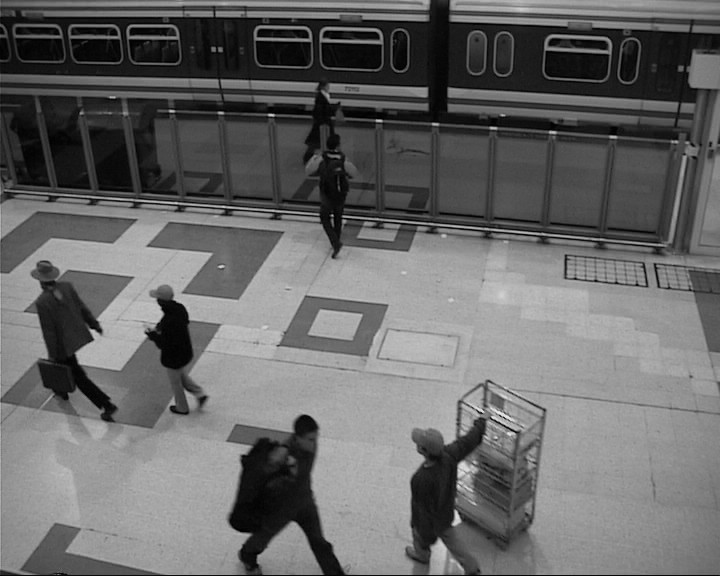
\includegraphics[width=\textwidth]{img/fd-frame.png}
	\end{minipage}
	\hfill
	\begin{minipage}[b]{0.49\textwidth}
		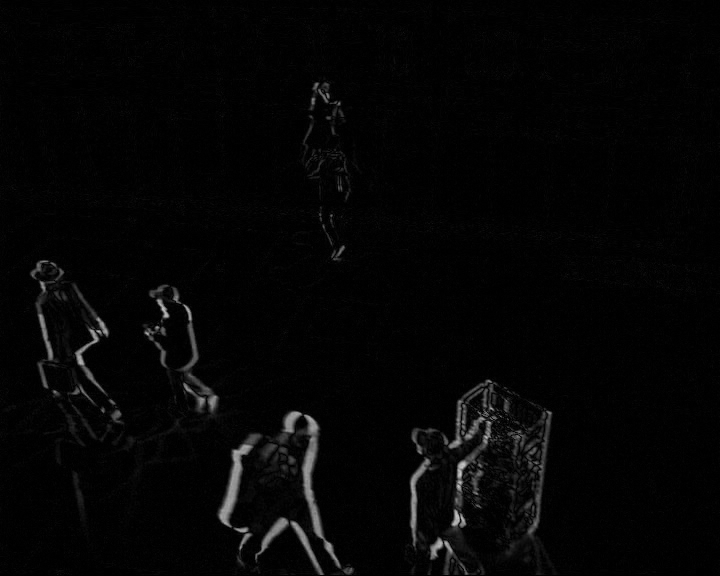
\includegraphics[width=\textwidth]{img/fd-diff.png}
	\end{minipage}
	\caption{Ramka obrazu i wyznaczona różnica ramek.}
	\label{fig:frame-difference-result}
\end{figure}
\section{Moduł generacji tła}

Poza najprostszymi przypadkami analizy ruchu, informacja uzyskana w wyniku odejmowania ramek sekwencji wizyjnej nie jest wystarczająca do analizy strumienia obrazów.
Zagadnienie to może być jednak elementem składowym bardziej rozbudowanych algorytmów, na przykład modułów realizujących algorytm generacji i modelowania tła, czy segmentacji obiektów pierwszoplanowych, gdzie pozwala określić zbiór obiektów będących w ruchu. 

Generacja tła to zadanie ekstrakcji elementów \textit{tła} badanego obrazu, a więc takich, które stanowią stały, niezmienny element sceny. 
Dzięki wydzieleniu obiektów tła, pozostałe elementy obrazu klasyfikowane są jako obiekty pierwszoplanowe. 
Zwykle, uważa się za nie elementy będące w ruchu. 
Uwzględnić jednak należy również obiekty, których ruch jest niejednostajny, na przykład zatrzymujący się piesi lub pojazdy na skrzyżowaniu.

Bardziej zaawansowane metody generacji tła uwzględniają ponadto dodatkowe warunki klasyfikacji obiektów do dwóch z omawianych grup:
\begin{itemize}
	\item cienie -- choć mogą być związane zarówno z elementami tła jak i pierwszoplanowymi, oczekiwane jest zwykle, by nie były uwzględniane w grupie obiektów wymagających analizy,
	\item ruchome elementy tła -- występujące na przykład pod wpływem wiatru ruchy roślin czy deszcz nie powinny być traktowane jako obiekty pierwszoplanowe,
	\item obiekty o niejednostajnym ruchu -- algorytm powinien klasyfikować poprawnie obiekty pierwszoplanowe, które pojawiają się na scenie a następnie zatrzymują, nie traktując ich jako elementy tła, 
	\item obiekty wzajemnie przesłaniające się -- elementy pierwszego planu mogą, w wyniku ruchu, zostać zasłonięte z perspektywy kamery przez elementy tła. Nie powinno to wpłynąć na zmianę klasyfikacji obiektów z obu grup.
	\item warunki oświetleniowe -- możliwość zmiany warunków oświetleniowych może wymagać ciągłej korekty parametrów generowanego modelu tła. Uwzględnić należy zarówno zmiany długookresowe, wynikające na przykład z cyklu dobowego, jak i krótkookresowe, wynikające z nagłych zmian, takich jak włączenie lub wyłączenie sztucznego oświetlenia sceny.
\end{itemize}

Zagadnienie modelowania tła nie jest trywialne i wymaga metod uwzględniających część lub wszystkie z wymienionych powyżej ograniczeń. 
Opracowanie dostępnej literatury poruszającej ten temat znaleźć można w pracy \cite{Kryjak2012}.
W ramach niniejszego opracowania zdecydowano się na realizację generacji tła przy pomocy metody średniej bieżącej, opisanej zależnością \eqref{eq:background-model}. 
Wartość modelu tła wyznaczana jest niezależnie dla każdej składowej obrazu.
\begin{equation}
\label{eq:background-model}
b^i(x,y) = \alpha p^i(x,y) + (1-\alpha)b^{i-1}(x,y)
\end{equation}
gdzie:
\begin{conditions}
	x,y & współrzędne piksela, \\
	i & indeks ramki w sekwencji obrazów, \\
	p^i(x,y) & wartość w $i$-tej ramce dla piksela o współrzędnych $(x,y)$, \\
	b^i(x,y) & wartość w $i$-tej ramce dla piksela modelu tła o współrzędnych $(x,y)$, \\
	\alpha & współczynnik bezwładności tła z przedziału $(0, 1]$. \\
\end{conditions}


Wadą przedstawionej metody jest jej wrażliwość na krótkookresowe zmiany oświetlenia.
Jednym ze sposobów eliminacji zakłóceń pojawiających się cyklicznie -- na przykład drgań liści pod wpływem wiatru -- jest wykorzystanie wielu niezależnie wyznaczanych modeli tła.
Stosując kilka modeli, budować można warianty dopasowane do najczęściej występujących przypadków, uporządkowanych według prawdopodobieństwa wystąpienia. 
Przy takim podejściu, obliczenia prowadzone są dla każdego modelu tła niezależnie, wartość nie jest jednak aktualizowana w sytuacji, gdy stan piksela nie jest zbliżony do oczekiwanego, związanego z wybranym modelem.
Jednym z dostępnych rozwiązań jest algorytm GMM (\emph{ang.} Gaussian Mixture Model), wykorzystujący kilka rozkładów prawdopodobieństwa Gaussa. 
W niniejszej pracy nie zdecydowano się na realizację opisanej powyżej metody eliminacji zakłóceń, uzasadniając to zachowaniem czytelności i prostoty implementacji.

Algorytm dostosowano do pracy z sygnałem opisanym w przestrzeni barw \textit{YCbCr}. 
Procedura generacji tła odbywa się niezależnie dla każdej składowej sygnału.
Przyjęto, że aktualizacja wartości modelu tła powinna mieć miejsce wyłącznie w przypadku, jeśli aktualnie badany piksel może być uznany za element tła. 
W tym celu wprowadzono dwa warunki wykonania obliczeń:
\begin{enumerate}
	\item Warunek ruchu.
	
	Aktualizacja powinna mieć miejsce wyłącznie w przypadku, jeśli wartość piksela nie uległa zmianie większej niż dopuszczalna względem poprzedniej ramki obrazu. 
	W przeciwnym razie przyjąć można, że nastąpił ruch elementu i piksel nie należy do tła.
	Zależność opisano wzorem \eqref{eq:background-model-movement-mask}.
	
	\begin{equation}
	\label{eq:background-model-movement-mask}
	d^i_Y(x,y) > T_{fd}
	\end{equation}
	gdzie:
	\begin{conditions}
		d^i_Y(x,y) & różnica ramek dla kanału $Y$ obrazu, opisana wzorem \eqref{eq:frame-difference}, \\ 
		T_{fd} & próg ruchu z zakresu $[0,255]$, zwykle nie przekraczający $30$. 
	\end{conditions}

	Większe wartości współczynnika $T_{fd}$ pozwalają dokonać aktualizacji modelu tła dla elementów o coraz większej różnicy względem poprzedniej ramki obrazu.
	
	\item Warunek tła.
	
	Aktualizacja powinna mieć miejsce wyłącznie w przypadku, jeśli piksel został sklasyfikowany jako element tła na bazie aktualnego modelu.
	Zależność opisano równaniem \eqref{eq:background-model-background-mask-1}.
	\begin{equation}
	\label{eq:background-model-background-mask-1}
	w_Ym^i_Y(x,y) + w_{Cb}m^i_{Cb}(x,y) + w_{Cr}m^i_{Cr}(x,y) > T_{bg}
	\end{equation}
	gdzie:
	\begin{conditions}
		m^i(x,y) & zmiana wartości piksela względem tła, opisana zależnością \eqref{eq:background-model-background-mask-2}, \\
		w_k & współczynnik wagi związany z $k$-tym kanałem \\
		T_{bg} & współczynnik bezwładności przynależności do tła z zakresu $[0,255]$. \\
	\end{conditions}
	
	\begin{equation}
	\label{eq:background-model-background-mask-2}
	m^i_k(x,y) = | p^i_k(x,y) - b^{i-1}_k(x,y)|
	\end{equation}
	gdzie:
	\begin{conditions}
		k & indeks składowej barwnej sygnału. \\ 

	\end{conditions}
	
	Większe wartości parametru $T_{bg}$ pozwalają na aktualizację modelu tła w sytuacji, gdy różnica piksela względem aktualnego modelu tła jest znaczna. 
	Jego wartość nie przekracza jednak zwykle $30$.
\end{enumerate}

W trakcie eksperymentów przyjęto wartości współczynników wag przynależności do tła odpowiednio: $w_Y=1, w_{Cb} = 2, w_{Cr} = 2$.
Aktualizacja modelu tła powinna mieć miejsce wyłącznie w sytuacji, gdy spełnione są oba warunki przedstawione powyżej.
Schemat blokowy algorytmu przestawiono na rysunku \ref{fig:background-model}.

\begin{figure}[h]
	\centering
	\def\svgwidth{\textwidth}
	\input{img/background-model.pdf_tex}
	\caption{Schemat architektury wyliczającej model tła.}
	\label{fig:background-model}
\end{figure}


Działanie modułu generacji tła przedstawiono na schemacie \ref{fig:background-model-impl}. 
Na wejściu, moduł otrzymuje aktualną wartość piksela w przestrzeni barw \textit{YCbCr} oraz poprzednią wartość piksela i modelu tła. 
Ponadto, przekazywane są parametry opisujące działanie algorytmu: $\alpha$, $T_{bg}$ oraz $T_{fd}$. 
Moduł odpowiedzialny jest za wyznaczenie maski obiektów tła oraz nowej wartości modelu, które stanowią wyjścia elementu obliczeniowego.

\begin{figure}[h]
	\centering
	\def\svgwidth{\textwidth}
	\input{img/background-model-impl.pdf_tex}
	\caption{Algorytm wyznaczania modelu tła.}
	\label{fig:background-model-impl}
\end{figure}

Algorytm wymaga wykorzystania dwóch buforów AXI VDMA. 
Jeden z nich przeznaczony jest do buforowania ramki obrazu wejściowego, natomiast drugi przechowuje aktualny model tła. 
Alternatywą jest zastosowanie wspólnego bufora i przechowywanie w nim dwóch scalonych sygnałów. 
Rozwiązanie to pozwala ograniczyć zapotrzebowanie na zasoby logiczne, może jednak wiązać się z trudnościami w synchronizacji wielu strumieni wizyjnych.

Algorytm zintegrowano z układem umożliwiającym komunikację z procesorem ARM, co pozwala na transmisję uzyskanego modelu tła i jego dalszą analizę. 
Wykorzystano w tym celu trzeci moduł AXI VDMA.
W praktycznych zastosowaniach moduł ten może okazać się zbędny, ze względu na to, że w jednym z pozostałych modułów VDMA przechowywany jest model tła dla poprzedniej klatki obrazu. 
Opóźnienie jednego cyklu nie powinno wpłynąć negatywnie na jakość działania aplikacji. 
Niezależny moduł VDMA pozwala jednak na przesyłanie wyników również w przypadku, gdy algorytm generacji tła nie stanowi ostatniego etapu obliczeń.


Ze względu na duże zapotrzebowanie algorytmu na elementy obliczeniowe logiki reprogramowalnej, zdecydowano się ograniczyć rozmiar kolejek FIFO do $64$ elementów.
Sprawdzono działanie aplikacji dla sygnału wizyjnego o rozdzielczości $1280 \times 720$ pikseli i częstotliwości sześćdziesięciu ramek na sekundę.
Szacowane zapotrzebowanie wynikowego systemu na energię elektryczną nie powinno przekroczyć $1,936W$. Właściwa energia wymagana do przeprowadzania operacji obliczeniowych nie przekracza wartości $1,797W$, w tym $1,565W$ ( $87\%$) to energia wymagana do obsługi układu ARM.


\begin{table}[!htb]
	\caption{Wykorzystanie zasobów przez aplikację.}
	\centering
	\label{tab;background-model-utilization}
	\begin{tabular}{|l|c|c|c|}
		\hline
		\textbf{Rodzaj zasobu} & \textbf{Użycie} & \textbf{Dostępne} & \textbf{Procent użycia}      \\ \hline
		FF                     & $6938$            & $17600$             & $39,42\%$                 \\ \hline
		LUT 6                  & $13670$            & $17600$             & $77,67\%$                 \\ \hline
		SLICE                  & $4400$            & $4400$             & $100\%$                 \\ \hline
		DSP 48                 & $15$               & $80$                & $18,75\%$                    \\ \hline
		BRAM                   & $12$               & $60$                & $20\%$                   \\ \hline
	\end{tabular}
\end{table}


W tabeli \ref{tab;background-model-utilization} przedstawiono zapotrzebowanie na zasoby FPGA układu Zynq.
Proporcjonalnie duże zużycie zasobów wynika z konieczności wykorzystania wielu modułów AXI VDMA oraz innych elementów wykorzystujących interfejs AXI. 
Może ono być ograniczone przez wykorzystanie jednego modułu do obsługi buforowania zarówno ramki obrazu, jak i modelu tła. 
W przypadku złożonych aplikacji, konieczne może okazać się użycie układu z większą liczbą dostępnych zasobów obliczeniowych. 
Moduł przeznaczony jest do pracy z częstotliwością $200MHz$, co pozwala na analizę sygnału wideo o rozdzielczości $1920 \times 1080$ pikseli i częstotliwości obrazu $60Hz$.
Wynik działania modelu programowego przedstawiono na rysunku \ref{fig:background-model-result}. Projekty Vivado i PetaLinux związane z omawianą aplikacją dodano jako załączniki do pracy oraz udostępniono w repozytorium \cite{git-repository}. Proces konfiguracji aplikacji przedstawiono w rozdziale \ref{sec:background-buffer-conf}.
\begin{figure}[H]
	\centering
	\begin{subfigure}[b]{0.49\textwidth}
		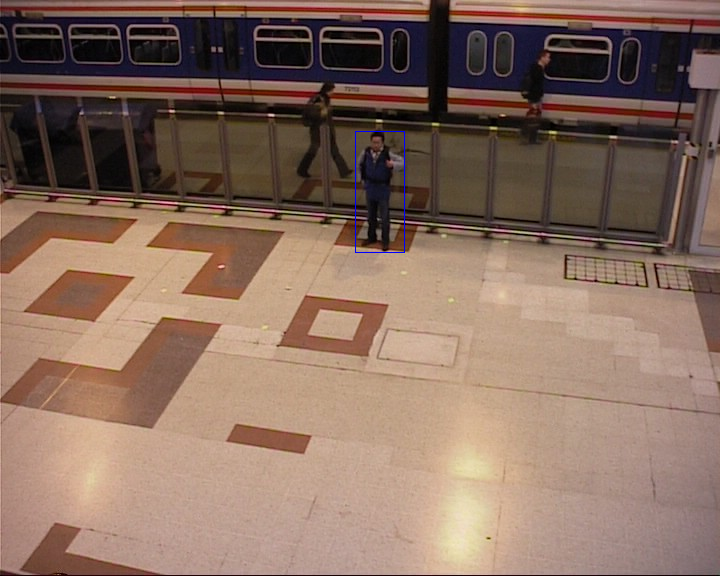
\includegraphics[width=\textwidth]{img/bg-input.png}
		\caption{Ramka obrazu.}
		\vspace{1ex}
	\end{subfigure}
	\hfill
	\begin{subfigure}[b]{0.49\textwidth}
		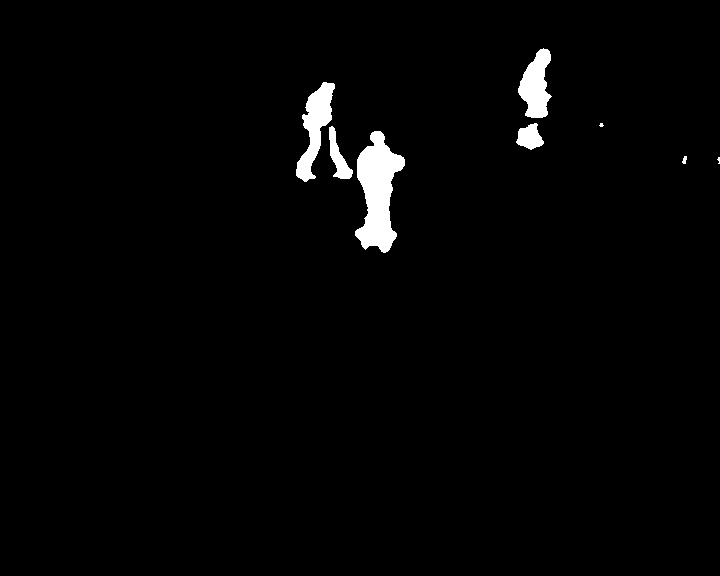
\includegraphics[width=\textwidth]{img/bg-fg.png}
		\caption{Maska obiektów pierwszoplanowych.}
		\vspace{1ex}
	\end{subfigure}

	\begin{subfigure}[b]{0.49\textwidth}
		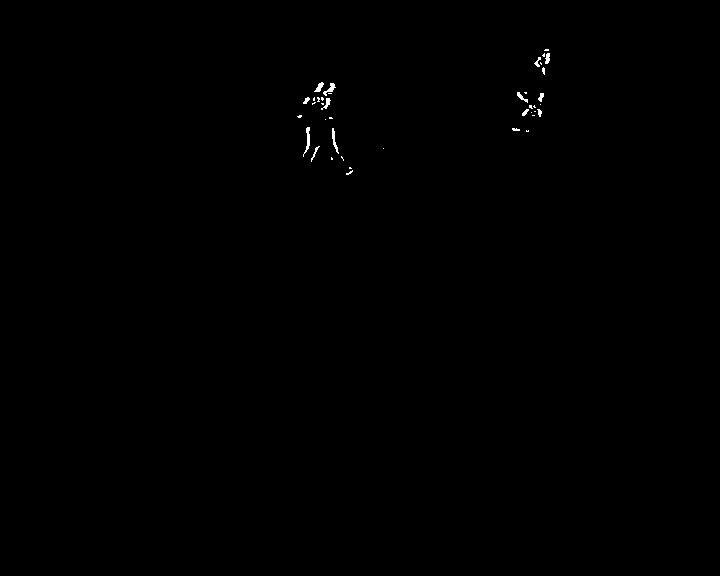
\includegraphics[width=\textwidth]{img/bg-mo.png}
		\caption{Maska ruchu.}
	\end{subfigure}
	\hfill
	\begin{subfigure}[b]{0.49\textwidth}
		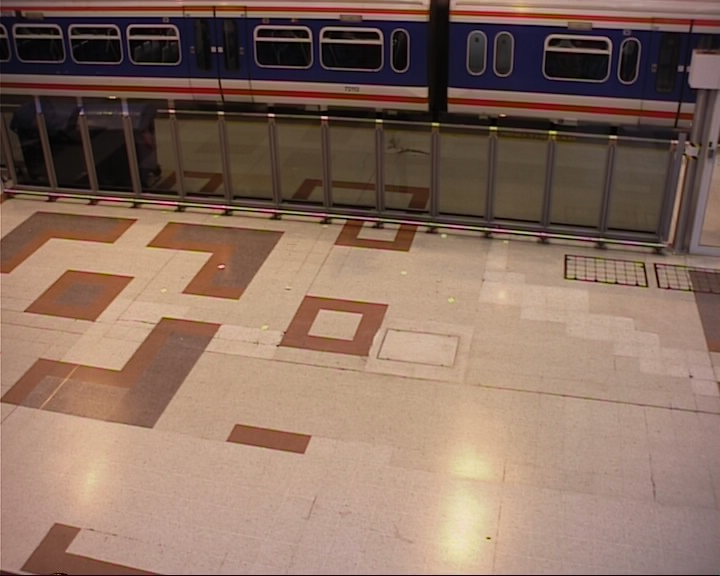
\includegraphics[width=\textwidth]{img/bg-model.png}
		\caption{Model tła.}
	\end{subfigure}
	\caption{Ramka obrazu wejściowego oraz wyznaczane przez model programowy obrazy masek i tła.}
	\label{fig:background-model-result}
\end{figure}

Dzięki zastosowaniu maski ruchu, obiekty poruszające się nie wpływają na stan modelu tła. Ponadto, dzięki badanu warunku przynależności do tła, osoba znajdująca się na pierwszym planie i nie będąca w ruchu również nie wpływa negatywnie na wynik działania algorytmu generacji tła.


%TODO 2. Uwagi podobnie jak wczęsniej tj.
%TODO może jakieś zdjęcie pokazuję, że działa. No i jeszcze te wszyskie szczegóły konfiguracji tego modułu. I coś o tym źródle - że ma to być film HD. Kolejna kwestia to przygotowanie takiego projektu - działającego/wzorcowego i do repo na płytce, a tu napisać, że takie coś jest.

%TODO Wydaje mi się, że jeszcze umawialiśmy się na przesył maski (kwestię indeksacji pozostawię) i coś po stronie PetaLiunx.
% co do indeksacji, nie sądzę, by moduł "zmieścił" się obok vdma na ZYBO. Musiałbym mocno zoptymalizować te struktury vdma, a wydaje mi się, że cenniejsza jest jednak czytelność tego, co mam teraz. Dlatego nie zająłem się indeksacją po stronie fpga. W CPU to w zasadzie wywołanie jednej metody w CV, ale nie ma szans na real-time.
% rzeczy po stronie peta opisałem w kolejnej sekcji.
% na wyjściu modułu dostępne są wartości maski, zaktualizowałem schemat

%TODO OK. A to są zdjęcie z modelu czy sprzętu. Bardziej wiarygodne byłoby z moniotrem :) I przy odejmowaniu ramek również. Ew. jeśli to jest png zapisany w peta to proszę to wyraźnie napisać.
% to zdjęcia z modelu progarmowego, sprecyzowałem. Impl. sprzętowa jest wciąż na etapie dynamicznego rozwoju, to znaczy regularnie przechodzę pomiędzy stanami działa/nie działa... Pracuję nad tym w wolnych chwilach, ale z tego powodu dodałem zrzuty z modelu.
% No i, oczywiście, było mi je znacznie wygodniej wygenerować w ten sposób. :)

\section{Integracja z systemem PetaLinux}

Na etapie prototypowania, elementy logiki reprogramowalnej kontrolowane były przez aplikację działającą w trybie \textit{bare-metal}, bez wsparcia dla systemu operacyjnego.
Po zakończeniu tego etapu, możliwe stało się zaprojektowanie aplikacji działającej pod kontrolą systemu PetaLinux, umożliwiającej wykorzystanie zaawansowanych funkcji systemu.
Założono, że projektowana aplikacja powinna spełniać szereg wymagań:

\begin{itemize}

	\item Konfiguracja modułów AXI i algorytmu.
	
	Podstawowym zadaniem aplikacji powinno być przeprowadzenie wstępnej konfiguracji modułów, wykorzystując w tym celu interfejs AXI. 
	Proces ten powinien mieć miejsce na etapie uruchamiania aplikacji. 
	Aplikacja powinna być też odpowiedzialna za przeprowadzenie procesu konfiguracji parametrów wykonywanego algorytmu wizyjnego.	
	Ponadto, działanie algorytmu nie powinno zostać przerwane w razie wyłączenia programu.
	
	\item Konfiguracja aplikacji przy użyciu argumentów wiersza poleceń.
	
	Konfiguracja parametrów działania aplikacji, w tym rozmiar przetwarzanych obrazów i parametry algorytmu powinny być konfigurowane przy użyciu argumentów wiersza poleceń.
	
	\item Monitorowanie działania algorytmu.
	
	Aplikacja powinna udostępniać opcję monitorowania stanu elementów algorytmu, ze szczególnym uwzględnieniem modułów AXI VDMA, odpowiedzialnych za buforowanie danych oraz komunikację z procesorem.
	
	\item Zapis wyników pracy algorytmu.
	
	Program powinien być odpowiedzialny za zapis wyników działania algorytmu, na przykład w formie obrazów przechowywanych w pamięci.
	
	\item Wykorzystanie komunikacji sieciowej.
	
	Uruchomienie aplikacji nie powinno wymagać fizycznego dostępu do układu Zynq. 
	Docelowym narzędziem komunikacji jest protokół SSH. 
	Ponadto, aplikacja powinna udostępniać interfejs wykorzystujący protokół HTTP, umożliwiający weryfikację stanu aplikacji przy użyciu przeglądarki internetowej.
	
	\item Kompatybilność z procedurami biblioteki OpenCV
	
	Aplikacja powinna zapewniać zgodność z technikami programowania wykorzystywanymi przez bibliotekę OpenCV w stopniu umożliwiającym użycie algorytmów biblioteki ze strukturami danych wykorzystywanymi przez program.
\end{itemize}

Zaprojektowano aplikację w języku C, spełniającą przedstawione wymagania.
Program odpowiedzialny jest za konfigurację elementów logiki reprogramowalnej na podstawie wartości przekazanych przy użyciu argumentów wiersza poleceń. 
Aplikacja wykonuje operacje monitorowania działania algorytmu i zapisu informacji logu do pliku. 
Ponadto, umożliwia cykliczny zapis obrazów będących wynikiem działania algorytmu do plików graficznych. 

Proces obsługi aplikacji opiera się na wykorzystaniu protokołu SSH, program udostępnia również interfejs HTTP, umożliwiający uzyskanie aktualnych wyników działania algorytmu.
Zbadano możliwość wykorzystania aplikacji w roli elementu obliczeniowego, odpowiedzialnego za przeprowadzenie części operacji algorytmicznych. 
Zaproponowano moduł indeksacji obiektów na bazie generowanego modelu tła. 
W tym celu wykorzystano procedurę \texttt{cv::connectedComponents} dostępną w bibliotece OpenCV. 

Ze względu na ograniczenia sprzętowe, moduł indeksacji nie był w stanie spełnić wymagań pracy w czasie rzeczywistym dla sygnału wizyjnego o częstotliwości $60Hz$ i rozdzielczości $1280 \times 720 $ pikseli -- jego wydajność nie przekraczała piętnastu ramek na sekundę.
Na rysunku \ref{fig:background-buffer-www} przedstawiono widok interfejsu \emph{www} udostępnianego przez aplikację, przedstawiający aktualny stan i wyniki działania programu. Interfejs wyświetla model tła oraz najnowszą ramkę obrazu, a także pokazuje wartości parametrów algorytmu i umożliwia ich modyfikację w trakcie działania aplikacji.
Związane z omawianą aplikacją projektu dodano jako załączniki do pracy oraz udostępniono w repozytorium \cite{git-repository}.
\begin{figure}[!htb]
	\centering
	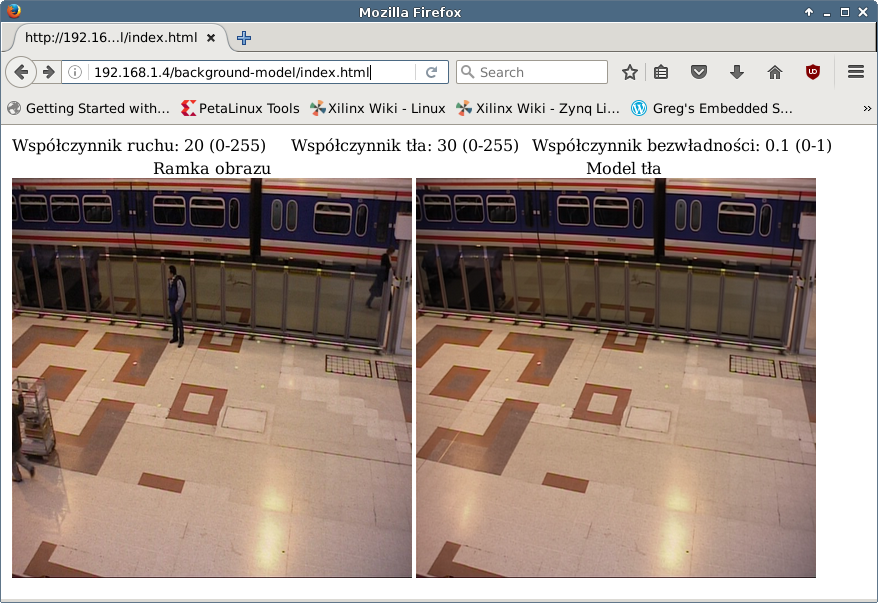
\includegraphics[width=12cm]{img/www-iface.png}
	\caption{Interfejs www aplikacji.}
	\label{fig:background-buffer-www}
\end{figure}
\section*{Podsumowanie}

Zaproponowane rozwiązania projektowe pozwalają na wykorzystanie części funkcji systemu operacyjnego, które badane były w ramach pracy. 
Szczególnie istotnym zagadnieniem jest komunikacja pomiędzy elementami zaprojektowanymi w dwóch architekturach. 
Dzięki wykorzystaniu transmisji danych, możliwe jest zaprojektowanie algorytmów podzielonych na moduły wykonywane naprzemiennie przez obie części układu, wykorzystując atuty obu architektur do możliwie maksymalnego zwiększenia wydajności pełnego algorytmu.

Ponadto, wykorzystanie systemu operacyjnego pozwala na realizację zadań zwykle niemożliwych w przypadku projektu aplikacji realizowanych wyłącznie przy użyciu elementów logiki reprogramowalnej lub sterowanych przez aplikację \textit{bare-metal}. 
Program działający pod kontrolą systemu operacyjnego umożliwia prowadzenie zadań konfiguracji, kontroli i monitorowania działania aplikacji z wykorzystaniem komunikacji sieciowej.

Wykorzystanie systemu operacyjnego pozwala również na implementację aplikacji w dowolnym języku programowania. 
Dzięki temu, stosując dedykowane rozwiązania programistyczne, projektowanie aplikacji o rozbudowanych możliwościach zajmuje mniej czasu.

W trakcie realizacji projektu napotkano szereg ograniczeń. 
\begin{itemize}
	\item Liczba elementów obliczeniowych wykorzystywanego układu Zynq nie pozwala na realizację rozbudowanych rozwiązań algorytmicznych przy użyciu zaproponowanych technik. 
	Ze względu na duże zapotrzebowanie na elementy logiki przez moduły AXI VDMA, buforowanie pełnych ramek obrazu jest kosztowne. 
	W przypadku bardziej rozbudowanych algorytmów, konieczne może być wykorzystanie układu o większych możliwościach lub zastosowanie technik optymalizacji zużycia zasobów.
	
	\item Procesor ARM dostępny w układzie Zynq nie pozwala na realizację algorytmów wizyjnych o dużej złożoności obliczeniowej w  czasie rzeczywistym. 
	Próba wykorzystania rozwiązań biblioteki OpenCV do indeksacji obiektów pierwszoplanowych nie spełniała ograniczeń czasowych dla sygnału o częstotliwości $60Hz$.
	
	W przypadku bardziej złożonych algorytmów, konieczne może być wykorzystanie układu o większej wydajności. 
	Innym rozwiązaniem może być użycie protokołów sieciowych do transmisji danych do elementu obliczeniowego oferującego wydajność wystarczającą do realizacji zadań obliczeniowych. 
	Dla zbioru algorytmów, których realizacja strumieniowa jest znana, możliwe jest również przeniesienie zadań obliczeniowych do elementów logiki reprogramowalnej. 
	W przypadku, gdy żadne z zaproponowanych rozwiązań nie jest możliwe, konieczne jest ograniczenie częstotliwości działania algorytmu do poziomu, dla którego układ obliczeniowy będzie spełniać ograniczenia czasowe.
	
	\item Proces budowy systemu operacyjnego na bazie projektu sprzętowego jest złożony i wymaga dużych nakładów czasowych. 
	Z tego powodu, na etapie projektowania połączeń logiki reprogramowalnej, wykorzystanie aplikacji typu \textit{bare-metal} pozwala skrócić okres prototypowania.
	
	W konsekwencji, konieczne może być zaprojektowanie dwóch aplikacji związanych z projektem: aplikacji \textit{bare-metal}, wykorzystywanej na etapie prototypu oraz programu działającego pod obsługą systemu operacyjnego, projektowanego po ukończeniu implementacji sprzętowej.
	
	Z tego powodu, aplikacje systemu operacyjnego nie pozwalają w pełni zastąpić programów \textit{bare-metal} i powinny być traktowane jako metoda rozbudowy możliwości projektu.
\end{itemize}

%TODO Tak samo jakieś screeny.
%TODO No i co z tego, że indeksacja 15 fps - a da się to jakoś pokazać ? Że to działa ? Wizualnie.
%TODO Co z HTTP ? 
% http -działa. Dołączę screen interfejsu, choć to będzie coś bardzo prostego. Tzn np aktualny wynik generacji tła czy indeksacji + gdzieś obok wartości parametrów algorytmu. Do tej pory zadowalałem się tym, że gdy uderzałem pod IP ZYBO dostawałem w odpowiedzi png z aktualnym stanem vdma, dlatego nie dodawałem tego do pracy.
% Myślałem o tym, by umożliwić modyfikację parametrów z poziomu http, ale serwer, który napisałem siedzi w C i podejrzewam, że dodanie obsługi parametrów zapytania będzie uciążliwa.

%TODO OK. No konfiguracja z http to byłoby już prawie smart camera :)
% hm...w sumie to dodałem teraz możliwość zmieniania wartości parametrów